\subsection{实验目的}
掌握一些基本的图像融合方法,包括基于像素灰度值的简单图像融合算法,以及彩色图像的分解于合成。完成遥感图像的图像融合。
\subsection{实验原理}
\subsubsection{图像融合的概念}
综合和提取两个或多个圆的图像信息,获得对同一场景或者目标更为准确、全面、可靠的图像,使之更适合人眼感知或计算机后续处理。
\begin{figure}[H]
	\centering
	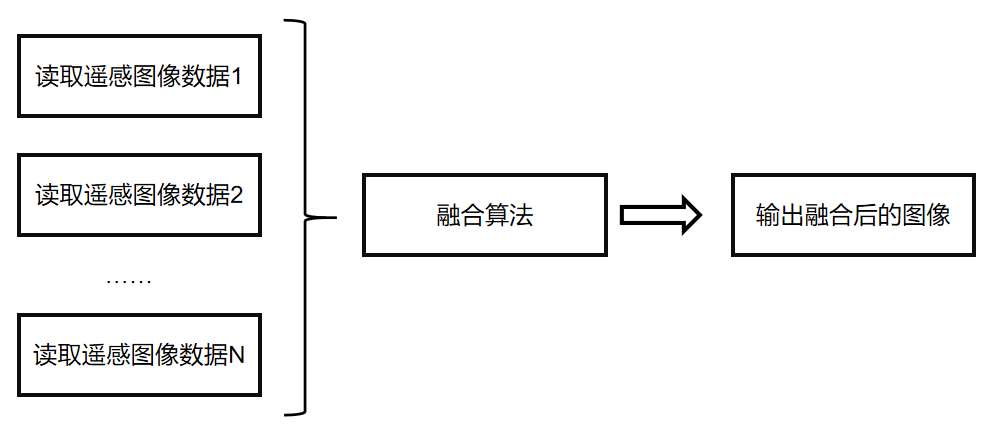
\includegraphics[width=0.7\linewidth]{figure/fusion_flowchart.png}
	\caption{图像融合算法流程图}
	\label{fig:fusion_flowchart}
\end{figure}
\subsubsection{简单的图像融合算法}
\begin{description}
	\item[像素灰度值平均或加权平均法]
	\[ I(x, y)=\frac{\sum_{n=1}^{N}W^n(x, y)I^n(x, y)}{\sum_{n=1}^{N}W^n(x, y)} \]
	\[ W^n(x, y)=\frac{1}{N} \]
	\item[像素灰度值选大法] 
	\[ I(x, y)=\max_n\{I^n(x, y),\quad n=1,2,\dots N\} \]
	\item[像素灰度值选小法] 
	\[ I(x, y)=\min_n\{I^n(x, y),\quad 1,2,\dots N\} \]
\end{description}
\subsubsection{彩色图像的分解与合成}
\begin{description}
	\item[能量图像] 
	\[ I=Ir+Ig+Ib \]
	\item[变换后的彩色图像合成]
	蓝色分量:加高斯噪声污染
	
	绿色分量:进行对数变换
	
	红色分量:进行图像反转
	
	重新合成彩色图像
\end{description}
\subsubsection{彩色图像合成}
通过图像变换与融合突出图像中感兴趣的目标。
\subsubsection{通过图像融合得到变化检测差异图}
\begin{description}
	\item[差异图像] 
	\[ I1=1-\min \left( \frac{\mu_1}{\mu_2},\frac{\mu_2}{\mu_1} \right)  \]
	\[ I2= \left| \log\frac{X_2}{X_1} \right| = \left| \log X_2 - \log X_1 \right|  \]
	\item[图像融合]
	两个差异图的低频成分平均融合,高频成分取小融合。
\end{description}
\subsection{实验流程}
\begin{figure}[H]
	\centering
	\begin{tikzpicture}[node distance=1.5cm]
	\node(start) [startstop] {开始};
	\node(inputimg) [io, below of=start] {读取图片};
	\node(separateimg) [process, below of=inputimg] {分离彩色图像颜色通道};
	\node(fusionchannels) [process, below of=separateimg] {加权合并各通道能量};
	\node(outputenergyimg) [io, below of=fusionchannels] {输出能量合成图像};
	\node(channelcompare) [process, below of=outputenergyimg] {使用图片的两个不同通道进行对比};
	\node(outputchannelcomparation) [io, below of=channelcompare] {输出比较的结果};
	\node(channeltransform) [process, below of=outputchannelcomparation] {对各个通道分别进行变换};
	\node(outputtransformed) [io, below of=channeltransform] {输出变换后的图像};
	\node(inputmask) [io, below of=outputtransformed] {输入兴趣区域蒙版};
	\node(interestedarea) [process, below of=inputmask] {合成兴趣区域图像};
	\node(outputinterestedarea) [io, below of=interestedarea] {输出兴趣区域图像};
	\node(end) [startstop, below of=outputinterestedarea] {结束};
	
	\draw[arrow] (start) -- (inputimg);
	\draw[arrow] (inputimg) -- (separateimg);
	\draw[arrow] (separateimg) -- (fusionchannels);
	\draw[arrow] (fusionchannels) -- (outputenergyimg);
	\draw[arrow] (outputenergyimg) -- (channelcompare);
	\draw[arrow] (channelcompare) -- (outputchannelcomparation);
	\draw[arrow] (outputchannelcomparation) -- (channeltransform);
	\draw[arrow] (channeltransform) -- (outputtransformed);
	\draw[arrow] (outputtransformed) -- (inputmask);
	\draw[arrow] (inputmask) -- (interestedarea);
	\draw[arrow] (interestedarea) -- (outputinterestedarea);
	\draw[arrow] (outputinterestedarea) -- (end);
	\end{tikzpicture}
\end{figure}
\subsection{实验程序}
\lstinputlisting[caption={简单像素加权融合程序}]{"../Executable Script/Exp 3/ColorImageEnergyGraph.m"}

\subsection{实验结果和分析}
\begin{figure}[H]
	\centering	
	\begin{minipage}{0.45\linewidth}
		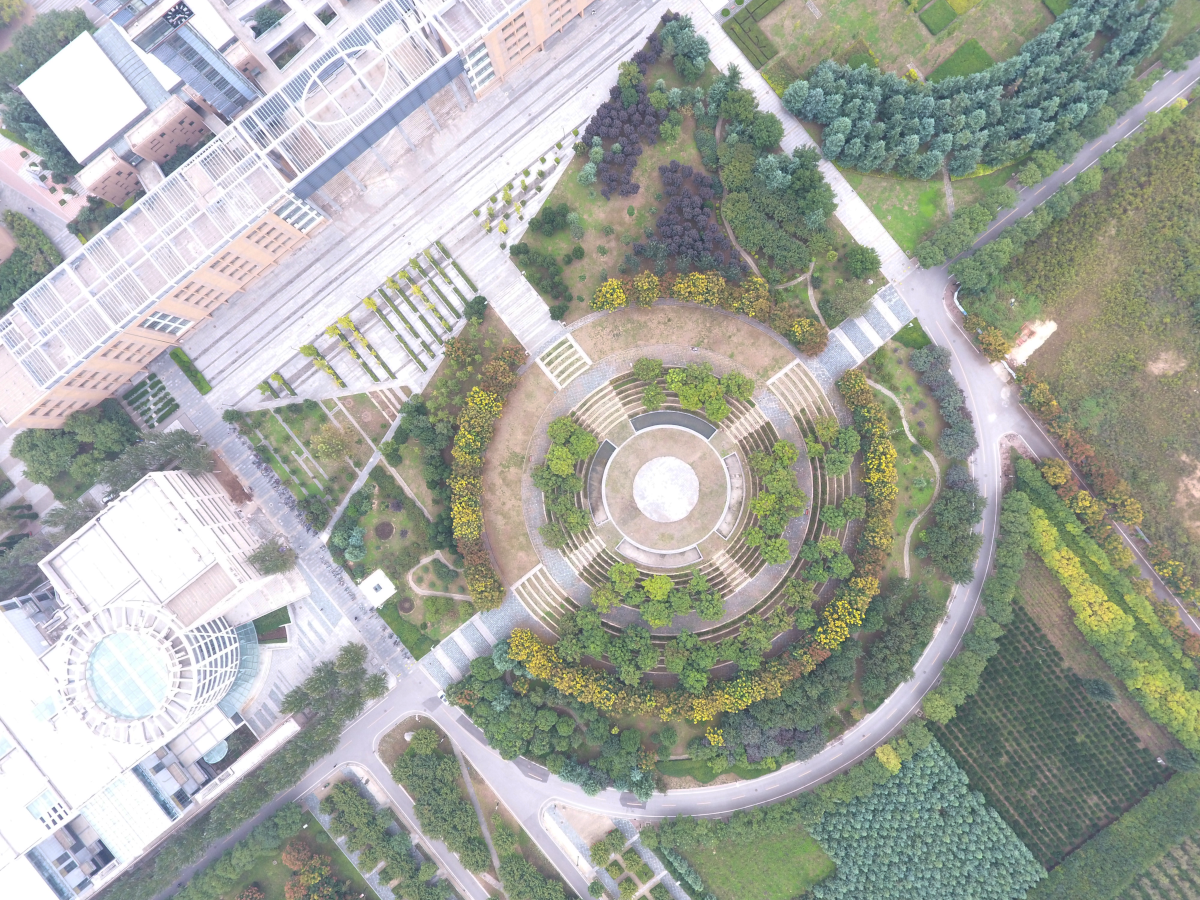
\includegraphics[width=\linewidth]{figure/DJI_0027_Compressed.png}
		\caption{原图片}
	\end{minipage}
	\begin{minipage}{0.45\linewidth}
		\includegraphics[width=\linewidth]{figure/DJI_0027_Energy.png}
		\caption{简单像素加权融合结果}
	\end{minipage}

\end{figure}